%% =============================================================================
%% chapters/appendix-provider-registry.tex
%% Appendix E: Implementation and Functional Specification for FHIR R5 Provider Registry Core Services
%% =============================================================================

\chapter{Provider Registry Core Services}
\label{app:provider_registry}
{\textit{\textbf{Implementation and Functional Specification for FHIR R5 Provider Registry Core Services}}}

\section{Overview \& Engineering Objectives}
\label{sec:pr_guide_overview}

Within modern regional and national healthcare ecosystems, maintaining an authoritative, synchronized, and referentially sound healthcare provider directory is critical to patient safety, clinical routing, electronic service discovery, and secure messaging. The \textbf{Harmonia FHIR R5 Provider Registry} provides an enterprise-grade, distributed provider directory subsystem embedded natively within the Harmonia Health Information Exchange (HIE) platform.

This specification serves as the authoritative architectural blueprint and functional manual for the Provider Registry core services suite, detailing:
\begin{enumerate}
    \item \textbf{Architectural Topology \& 5-Tier Interaction Model}: The design separating synchronous read/search data paths from asynchronous governed change pipelines.
    \item \textbf{FHIR R5 Resource Model \& Relationship Topology}: First-class management and relationship graph traversal across seven core resources: \texttt{Practitioner}, \texttt{PractitionerRole}, \texttt{Organization}, \texttt{Location}, \texttt{HealthcareService}, \texttt{Endpoint}, and \texttt{Group}.
    \item \textbf{REST API Gateway Contract \& Interaction Matrix}: Exact HTTP verbs, request/response payloads, status codes, search parameters, dynamic \texttt{CapabilityStatement} generation (\texttt{GET /metadata}), and asynchronous status polling (\texttt{GET /Task/\{id\}}).
    \item \textbf{Governed Change Processing Lifecycle \& Pragma State Machine}: Event-driven write ingestion, state transitions (\texttt{RECEIVED} $\rightarrow$ \texttt{VALIDATING} $\rightarrow$ \texttt{APPROVED} $\rightarrow$ \texttt{COMMITTING} $\rightarrow$ \texttt{COMPLETED} or \texttt{REJECTED}), audit checkpoints, and structured \texttt{OperationOutcome} diagnostics.
    \item \textbf{Per-Resource Ergon Processing Activities \& Referential Integrity Engine}: The 7 dedicated per-resource Ergon activities, reference validation rules, duplicate identifier detection, and Apache Camel pipeline routing.
    \item \textbf{Authoritative Persistence, Optimistic Concurrency \& Versioning}: PostgreSQL relational document storage (\texttt{hie\_fhir\_resources}), monotonic version incrementing, and \texttt{If-Match}/\texttt{ETag} conflict protection.
    \item \textbf{Security, RBAC \& Resource-Level Authorization}: Granular permission scopes, token inspection, and security interceptor mechanics.
    \item \textbf{Paradeigma Exemplar Generation \& Automated Verification Testbed}: Synthetic graph generation, acceptance test suites, concurrency collision testing, and crash-recovery verification.
\end{enumerate}

% =============================================================================
% SECTION E.2: ARCHITECTURAL TOPOLOGY & 5-TIER INTERACTION MODEL
% =============================================================================
\section{Architectural Topology \& 5-Tier Interaction Model}
\label{sec:pr_topology}

Harmonia enforces a fundamental architectural dichotomy between \textbf{Synchronous Read/Search Pathways} and \textbf{Asynchronous Governed Write Pathways}:

\begin{principlebox}{The Governed Change Invariant}
HTTP \texttt{POST} (create) and \texttt{PUT} (update) interactions on provider directory endpoints are treated strictly as \textbf{Requests for Change}, not immediate mutation instructions. Authoritative state is never mutated synchronously inside the HTTP request thread. All mutations must be verified, referentially checked, approved, and persisted asynchronously through the \texttt{Energeia} workflow engine.
\end{principlebox}

\subsection{Synchronous Read and Search Data Path}
When an external clinical application, hospital EHR, or clinician user interface queries provider information (e.g. \texttt{GET /Practitioner/123} or \texttt{GET /PractitionerRole?organization=Org-1}):
\begin{enumerate}
    \item \textbf{Edge Ingestion (\texttt{pylai-fhir-registry})}: The request hits the \texttt{FhirRestGatewayController} on port \texttt{8089}.
    \item \textbf{Authentication \& Authorization}: The \texttt{FhirSecurityInterceptor} validates the bearer token/headers and delegates to \texttt{ThemisService} to evaluate \texttt{ProviderRegistryReadPolicy} (verifying caller has authority \texttt{provider.read} or role \texttt{PRV\_RDR}).
    \item \textbf{Direct Persistence Delegation}: The controller bypasses messaging queues and invokes \texttt{FhirStorageService} in \texttt{hestia/mnemosyne-clinical} directly.
    \item \textbf{Relational Query Execution}: Indexed SQL lookups execute against \texttt{hie\_fhir\_resources}, returning the active FHIR JSON resource or search \texttt{Bundle} in sub-50 milliseconds with \texttt{HTTP 200 OK}.
\end{enumerate}

\subsection{Asynchronous Governed Change Path}
When an external administration portal, credentialing service, or master file interface submits a modification (e.g. \texttt{POST /Practitioner} or \texttt{PUT /PractitionerRole/PRR-1}):
\begin{enumerate}
    \item \textbf{Gateway Ingestion}: \texttt{FhirRestGatewayController} authenticates the caller and performs structural JSON parsing and schema validation.
    \item \textbf{Pragma Envelope Creation}: \texttt{ChangeRequestSubmissionService} constructs a canonical \texttt{ProviderRegistryChangePragma} with status \texttt{ACCEPTED}, recording the submitted resource, requester, source system, and \texttt{If-Match} version preconditions.
    \item \textbf{Durable Queue Dispatch}: The gateway dispatches a \texttt{PetasosMessage} to Apache ActiveMQ Artemis queue \texttt{harmonia.provider.registry.change.request} and immediately returns \texttt{HTTP 202 Accepted} with header \texttt{Location: /Task/\{pragmaId\}}.
    \item \textbf{Workflow Ingestion \& Sequencing}: Ponos consumes the message and instantiates the Praxis sequence \texttt{seq-provider-registry-change-pipeline}.
    \item \textbf{Ergon Verification}: The designated resource Ergon (e.g. \texttt{PractitionerRoleChangeErgon}) invokes \texttt{ProviderRegistryReferenceValidator} to verify that all referenced target entities exist and are active in Mnemosyne.
    \item \textbf{Commit \& Versioning}: Upon successful validation, the resource is committed to Mnemosyne PostgreSQL, incrementing its \texttt{version\_id}. The underlying \texttt{Pragma} transitions to \texttt{COMPLETED}, and the updated resource becomes immediately visible to subsequent read/search requests.
\end{enumerate}

% =============================================================================
% SECTION E.3: FHIR R5 PROVIDER REGISTRY RESOURCE MODEL
% =============================================================================
\section{FHIR R5 Provider Registry Resource Model \& Relationship Topology}
\label{sec:pr_resource_model}

The Harmonia Provider Registry models the healthcare delivery enterprise across seven first-class FHIR R5 resources, adhering strictly to official HL7 FHIR Release 5 definitions:

\begin{table}[htbp]
\centering
\small
\begin{tabularx}{\textwidth}{l p{3.2cm} X}
\toprule
\textbf{Resource Type} & \textbf{Core Identity} & \textbf{Domain Function \& Structural Relationships} \\
\midrule
\texttt{Practitioner} & Individual & Individual healthcare practitioner (physician, surgeon, nurse, allied health). Holds legal names, professional qualifications, and deterministic identifiers (HPI-I, NPI, AHPRA). \\
\addlinespace
\texttt{PractitionerRole} & Association Link & Core relationship binding a \texttt{Practitioner} to an \texttt{Organization}, operating at specific physical \texttt{Location}(s), providing specific \texttt{HealthcareService}(s), and reachable via technical \texttt{Endpoint}(s). \\
\addlinespace
\texttt{Organization} & Legal Entity & Healthcare provider organization, hospital network, clinic, or diagnostic trust. Holds national identifiers (HPI-O), parent/child hierarchies, and administrative contacts. \\
\addlinespace
\texttt{Location} & Physical Facility & Physical or virtual site of healthcare delivery (hospital ward, clinic suite, operating theatre). References managing \texttt{Organization} and communication \texttt{Endpoint}(s). \\
\addlinespace
\texttt{HealthcareService} & Clinical Offering & Clinical service or specialty delivered by an organization (e.g. Inpatient Cardiology, Emergency Triage). References offering \texttt{Organization} and operating \texttt{Location}(s). \\
\addlinespace
\texttt{Endpoint} & Electronic Channel & Independent technical communication destination (FHIR REST, secure messaging, MLLP, Direct). Holds connection type codings, address URLs, and managing \texttt{Organization}. \\
\addlinespace
\texttt{Group} & Cohort / Specialty & Logical grouping of practitioners, organizations, or related healthcare entities for multidisciplinary teams, on-call rosters, or clinical specialties. \\
\bottomrule
\end{tabularx}
\caption{FHIR R5 Provider Registry Managed Resource Model Catalog}
\label{tab:pr_resource_catalog}
\end{table}

\subsection{Relationship Graph and Referential Topology}
Figure~\ref{fig:pr_graph_topology} illustrates the interconnected relationship topology enforced across the seven directory resource types.

\begin{figure}[htbp]
\centering
%\small
%\begin{verbatim}
%                           +------------------+
%                           |   Practitioner   |
%                           +--------+---------+
%                                    | 1..*
%                                    v
%                           +------------------+
%              +----------->| PractitionerRole |<-----------+
%              |            +----+----+---+----+            |
%              | 1..*            |    |   |            1..* |
%              v                 |    |   +-----------------+----------+
%     +-----------------+        |    |                     |          |
%     |  Organization   |<-------+    v                     v          v
%     +--------+--------+      +------------+      +-------------+ +----------+
%              | 1..*          |  Location  |      | Healthcare  | | Endpoint |
%              +-------------->+------+-----+      |   Service   | +----------+
%                                     | 1..*       +------+------+
%                                     v                   | 1..*
%                              +------------+             |
%                              |  Endpoint  |<------------+
%                              +------------+
%
%                                 +-------+
%                                 | Group |----> [ Practitioner | Organization ]
%                                 +-------+
%\end{verbatim}
	\setlength{\fboxrule}{0.5pt}
	\setlength{\fboxsep}{3pt}
	\fbox{%
		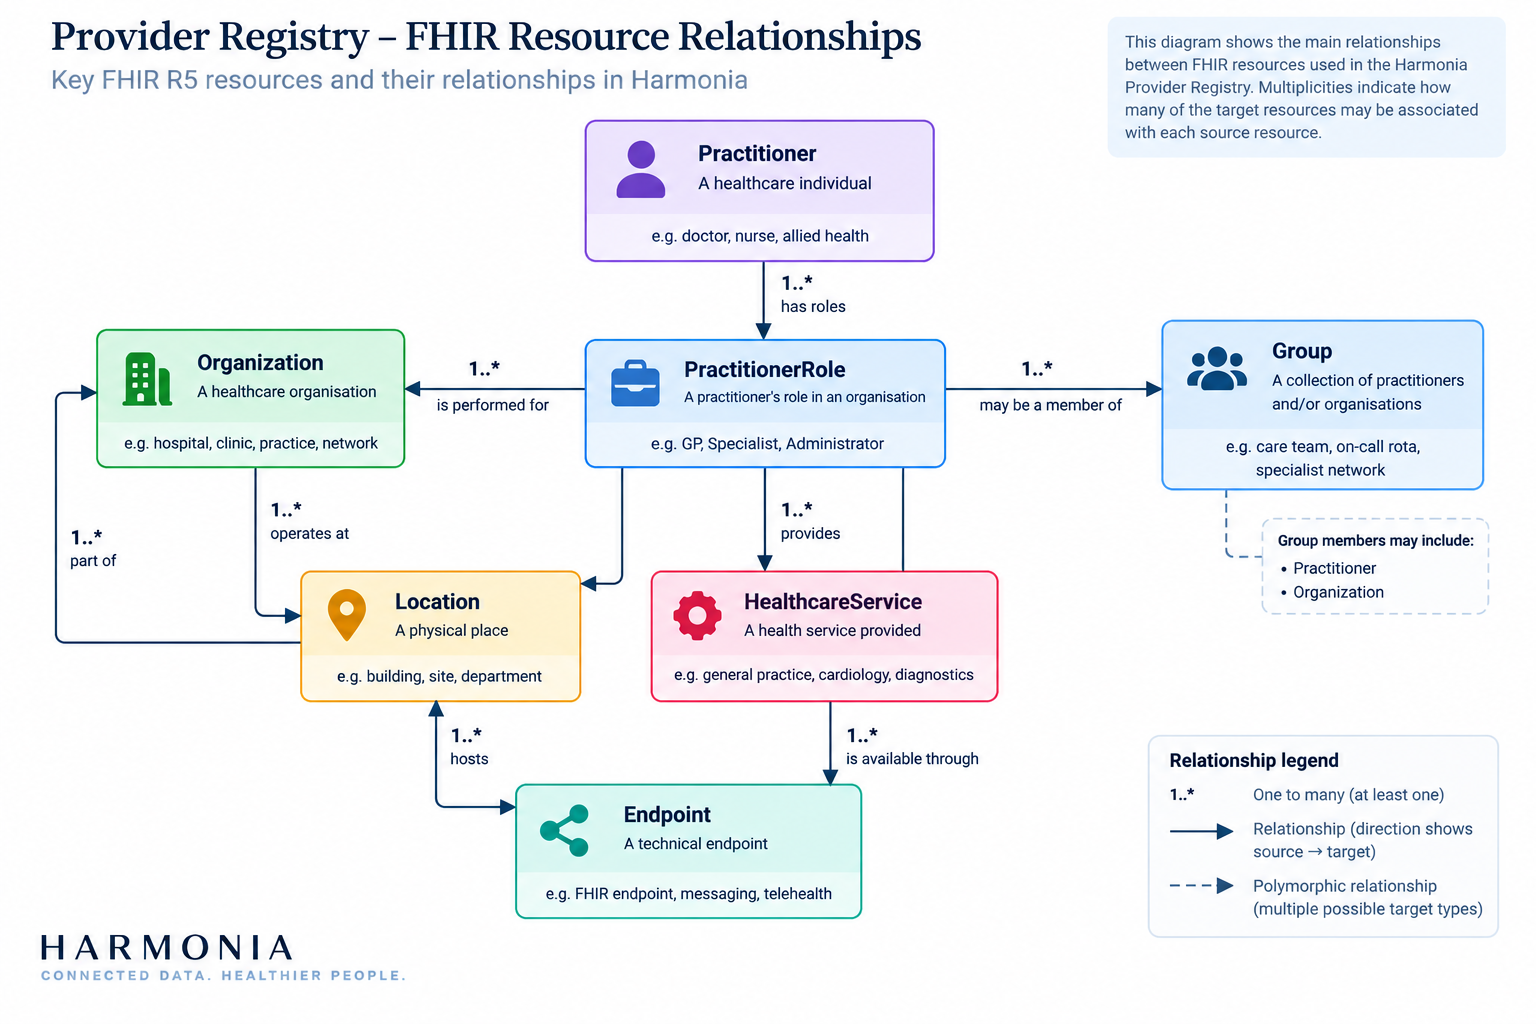
\includegraphics[width=0.94\textwidth, height=0.82\textheight,keepaspectratio]
		{images/fhir-r5-provider-registry-entity-relationship-and-referential-dependency-graph.png}
	}
	\caption{FHIR R5 Provider Registry Entity Relationship and Referential Dependency Graph}
	\label{fig:pr_graph_topology}
\end{figure}

\subsection{Endpoint as an Independent First-Class Entity}
In accordance with architectural standards, \texttt{Endpoint} is modeled and persisted strictly as an independent FHIR resource rather than an embedded string property on PractitionerRole. This allows multiple organizations, facilities, and practitioner roles to share electronic endpoints, support certificate rotation, and manage technical communication parameters (e.g., encryption protocols, payload MIME types, TLS certificates) centrally without duplicating configuration across clinical records.

% =============================================================================
% SECTION E.4: REST API GATEWAY CONTRACT & INTERACTION MATRIX
% =============================================================================
\section{REST API Gateway Contract \& Interaction Matrix}
\label{sec:pr_api_contract}

The \texttt{pylai-fhir-registry} gateway exposes standard FHIR R5 REST endpoints across all seven directory resources plus the \texttt{Task} and \texttt{metadata} operations:

\begin{table}[htbp]
\centering
\small
\begin{tabularx}{\textwidth}{l l p{3.5cm} l X}
\toprule
\textbf{Interaction} & \textbf{Verb} & \textbf{Path / URI} & \textbf{Mode} & \textbf{HTTP Response Codes} \\
\midrule
Read & \texttt{GET} & \texttt{/\{Resource\}/\{id\}} & Synchronous & \texttt{200 OK}, \texttt{404 Not Found}, \texttt{410 Gone} \\
Search & \texttt{GET} & \texttt{/\{Resource\}?\{params\}} & Synchronous & \texttt{200 OK} (\texttt{Bundle}) \\
Create Request & \texttt{POST} & \texttt{/\{Resource\}} & Asynchronous & \texttt{202 Accepted} (\texttt{Location: /Task/\{id\}}), \texttt{400 Bad Request} \\
Update Request & \texttt{PUT} & \texttt{/\{Resource\}/\{id\}} & Asynchronous & \texttt{202 Accepted} (\texttt{Location: /Task/\{id\}}), \texttt{412 Precondition Failed} \\
Task Polling & \texttt{GET} & \texttt{/Task/\{id\}} & Synchronous & \texttt{200 OK} (\texttt{Task}), \texttt{404 Not Found} \\
Metadata & \texttt{GET} & \texttt{/metadata} & Synchronous & \texttt{200 OK} (\texttt{CapabilityStatement}) \\
\bottomrule
\end{tabularx}
\caption{FHIR R5 Provider Registry REST Interaction Matrix}
\label{tab:pr_interaction_matrix}
\end{table}

\subsection{Multi-Parameter Search Capabilities}
The \texttt{FhirStorageService} in Mnemosyne executes multi-parameter search queries supporting standard FHIR search parameters:

\begin{itemize}
    \item \textbf{\texttt{Practitioner}}: \texttt{\_id}, \texttt{identifier} (HPI-I, NPI), \texttt{name} (family, given), \texttt{active}.
    \item \textbf{\texttt{PractitionerRole}}: \texttt{\_id}, \texttt{identifier}, \texttt{practitioner} (reference), \texttt{organization} (reference), \texttt{location} (reference), \texttt{service} (reference), \texttt{active}.
    \item \textbf{\texttt{Organization}}: \texttt{\_id}, \texttt{identifier} (HPI-O), \texttt{name}, \texttt{active}.
    \item \textbf{\texttt{Location}}: \texttt{\_id}, \texttt{identifier}, \texttt{name}, \texttt{organization} (managing organization reference), \texttt{status}.
    \item \textbf{\texttt{HealthcareService}}: \texttt{\_id}, \texttt{identifier}, \texttt{name}, \texttt{organization} (provided-by reference), \texttt{location} (operating site reference), \texttt{active}.
    \item \textbf{\texttt{Endpoint}}: \texttt{\_id}, \texttt{identifier}, \texttt{name}, \texttt{organization} (managing organization reference), \texttt{status}, \texttt{connection-type}.
    \item \textbf{\texttt{Group}}: \texttt{\_id}, \texttt{identifier}, \texttt{name}, \texttt{type}, \texttt{actual} (membership mode: \texttt{true}/\texttt{false}).
\end{itemize}

\subsection{CapabilityStatement Specification (\texttt{GET /metadata})}
The \texttt{CapabilityStatementProvider} dynamically builds an official FHIR R5 \texttt{CapabilityStatement} describing:
\begin{itemize}
    \item FHIR Release \texttt{5.0.0}.
    \item REST server mode with full resource descriptions for all 7 directory types plus \texttt{Task}.
    \item Advertised interactions (\texttt{read}, \texttt{search-type}, \texttt{create}, \texttt{update}).
    \item Exact supported search parameters per resource type.
    \item Security service configuration (\texttt{OAuth2} / \texttt{Bearer} token authentication).
\end{itemize}

\subsection{Asynchronous Task Polling (\texttt{GET /Task/\{id\}})}
When a client polls \texttt{GET /Task/\{id\}}, the \texttt{ProviderRegistryTaskResourceProvider} maps internal \texttt{Pragma} state directly to standard FHIR \texttt{Task} elements:
\begin{itemize}
    \item \texttt{Task.status}: Mapped from \texttt{PragmaStatus} (\texttt{requested} $\rightarrow$ \texttt{in-progress} $\rightarrow$ \texttt{completed} or \texttt{failed}).
    \item \texttt{Task.focus}: References the requested target resource (e.g. \texttt{PractitionerRole/PRR-101}).
    \item \texttt{Task.output}: Upon successful completion, embeds a reference to the persisted resource and resulting version (e.g. \texttt{Practitioner/P-100/\_history/2}). On failure, embeds the diagnostic \texttt{OperationOutcome}.
\end{itemize}

% =============================================================================
% SECTION E.5: GOVERNED CHANGE PROCESSING LIFECYCLE
% =============================================================================
\section{Governed Change Processing Lifecycle \& Pragma State Machine}
\label{sec:pr_lifecycle}

Every asynchronous change request progresses through a deterministic persistent state machine tracked across \texttt{PragmaCheckpoint} records in the \texttt{Mneme} distributed cache and \texttt{Mnemosyne} relational database:

%\begin{lstlisting}[language=bash, caption={Provider Registry Change Request State Progression}]
%+--------------------------------------------------------------------------+
%|                               [ RECEIVED ]                               |
%|               (Gateway validates JSON structure & creates Pragma)        |
%+------------------------------------+-------------------------------------+
%                                     |
%                                     v
%+--------------------------------------------------------------------------+
%|                              [ VALIDATING ]                              |
%|           (Ergon activity executes reference & business checks)          |
%+-------------------+----------------------------------+-------------------+
%                    |                                  |
%           [Validation Failed]                [Validation Passed]
%                    |                                  |
%                    v                                  v
%+---------------------------------------+  +-------------------------------+
%|             [ REJECTED ]              |  |         [ APPROVED ]          |
%|    (Embeds OperationOutcome PR-VAL-*) |  |  (Automatic or Steward Pass)  |
%+---------------------------------------+  +---------------+---------------+
%                                                           |
%                                                           v
%+--------------------------------------------------------------------------+
%|                              [ COMMITTING ]                              |
%|        (Persisting resource to Mnemosyne PostgreSQL & incrementing ver)  |
%+------------------------------------+-------------------------------------+
%                                     |
%                                     v
%+--------------------------------------------------------------------------+
%|                              [ COMPLETED ]                               |
%|        (Resource available for GET/SEARCH; Task status set to completed) |
%+--------------------------------------------------------------------------+
%\end{lstlisting}

\begin{figure}
	\setlength{\fboxrule}{0.5pt}
	\setlength{\fboxsep}{3pt}
    \centering
    \fbox{%
		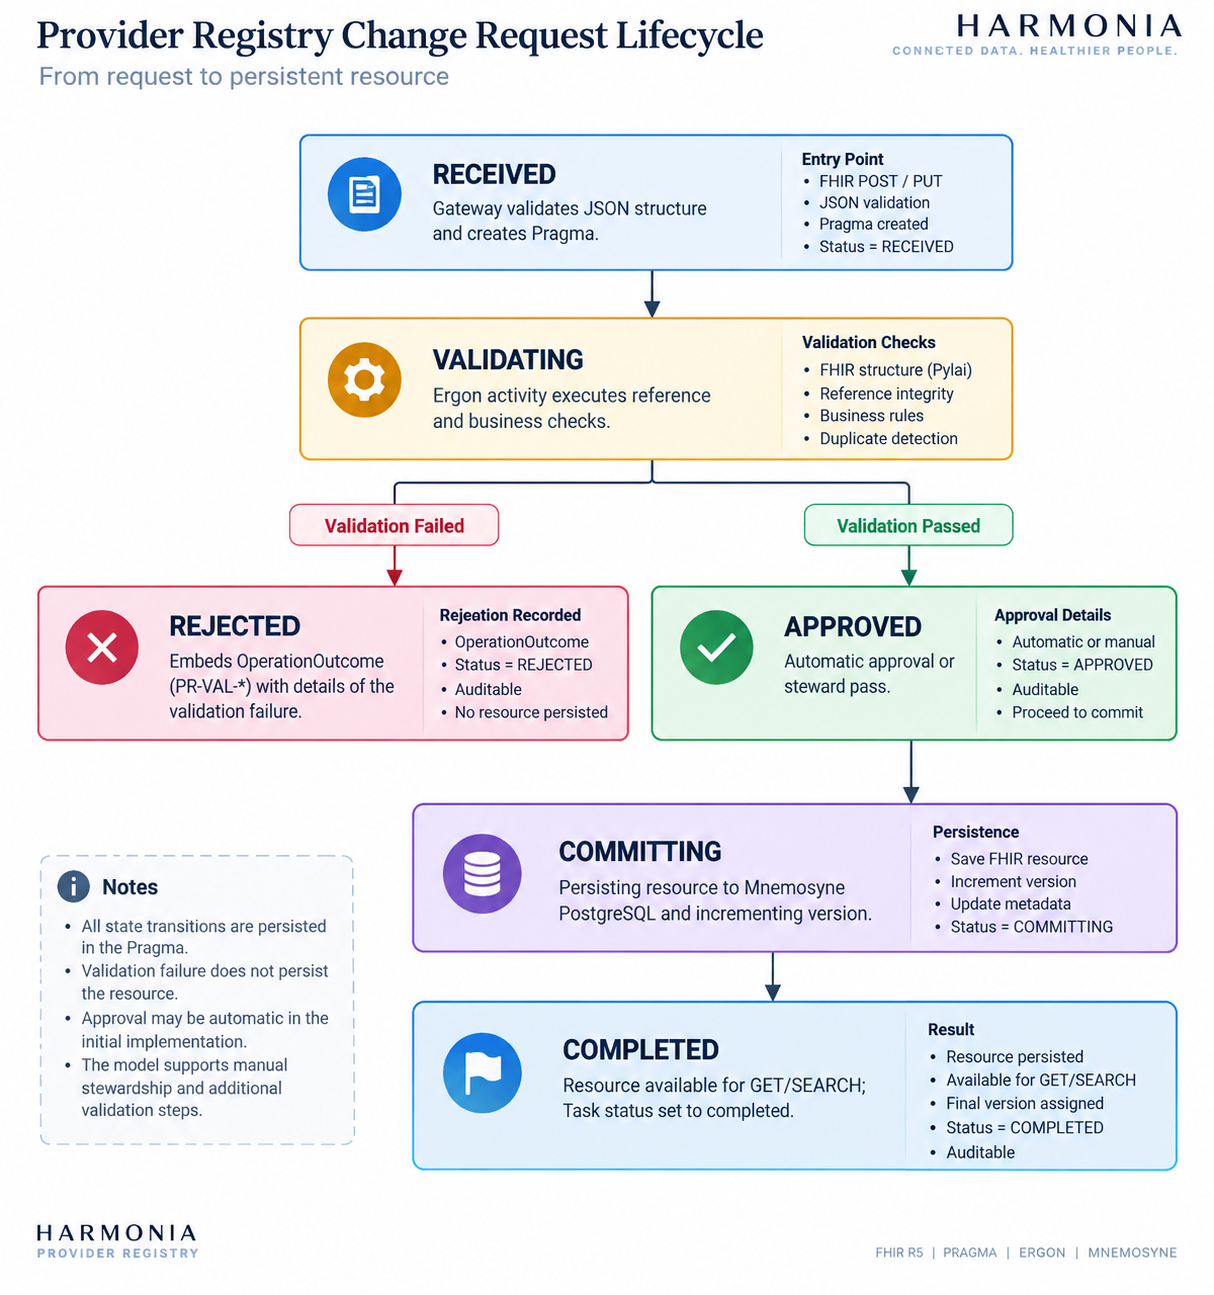
\includegraphics[width=0.94\textwidth, height=0.82\textheight,keepaspectratio]
		{images/provider-registry-change-request-state-progression.png}
	}
	\caption{Provider Registry Change Request State Progression}
	\label{fig:provider-registry-change-lifecycle}
\end{figure}

\subsection{State Machine Transition Rules}
\begin{description}
    \item[\texttt{RECEIVED} $\rightarrow$ \texttt{VALIDATING}]: Triggered when the Ponos WorkEngine consumes the change task from ActiveMQ Artemis and routes to the dedicated resource Ergon activity.
    \item[\texttt{VALIDATING} $\rightarrow$ \texttt{REJECTED}]: Fired when the submitted resource references non-existent or inactive resources, contains duplicate deterministic identifiers, or fails business schema rules. An \texttt{OperationOutcome} is generated and attached to the task output.
    \item[\texttt{VALIDATING} $\rightarrow$ \texttt{APPROVED}]: In the first iteration, change requests that pass all structural, referential, and uniqueness checks are automatically approved. The architecture includes extension hooks for human steward approval workflows.
    \item[\texttt{APPROVED} $\rightarrow$ \texttt{COMMITTING}]: The Ergon persists the approved resource into \texttt{hie\_fhir\_resources}, incrementing the \texttt{version\_id} and stamping \texttt{last\_updated}.
    \item[\texttt{COMMITTING} $\rightarrow$ \texttt{COMPLETED}]: Terminal success milestone. Checkpoints are synchronized, and the task output references the newly persisted resource version.
\end{description}

% =============================================================================
% SECTION E.6: PER-RESOURCE ERGON ACTIVITIES & REFERENTIAL INTEGRITY
% =============================================================================
\section{Per-Resource Ergon Processing Activities \& Referential Integrity Engine}
\label{sec:pr_erga_reference}

Harmonia implements dedicated, strongly-typed Ergon activities extending \texttt{ErgonBase} for each resource type:

\begin{table}[htbp]
\centering
\small
\begin{tabularx}{\textwidth}{l p{4.0cm} X}
\toprule
\textbf{Ergon Activity Class} & \textbf{Target Resource} & \textbf{Specialized Validation \& Verification Responsibilities} \\
\midrule
\texttt{PractitionerChangeErgon} & \texttt{Practitioner} & Validates legal human name, gender, qualifications, and checks duplicate deterministic HPI-I / NPI identifiers in Mnemosyne. \\
\addlinespace
\texttt{PractitionerRoleChangeErgon} & \texttt{PractitionerRole} & Performs deep referential verification ensuring target \texttt{Practitioner}, \texttt{Organization}, \texttt{Location}(s), \texttt{HealthcareService}(s), and \texttt{Endpoint}(s) exist and are active. \\
\addlinespace
\texttt{OrganizationChangeErgon} & \texttt{Organization} & Validates organization name, active status, national identifier (HPI-O), and validates parent organization hierarchy references. \\
\addlinespace
\texttt{LocationChangeErgon} & \texttt{Location} & Validates facility coordinates, addresses, operational status, and verifies managing organization reference existence. \\
\addlinespace
\texttt{HealthcareServiceChangeErgon} & \texttt{HealthcareService} & Validates specialty codes, active status, and verifies provided-by organization and location references. \\
\addlinespace
\texttt{EndpointChangeErgon} & \texttt{Endpoint} & Validates connection type coding, address URL structure, supported payload MIME types, and managing organization reference. \\
\addlinespace
\texttt{GroupChangeErgon} & \texttt{Group} & Validates group membership type (definitional vs actual), member count, and verifies individual member entity references. \\
\bottomrule
\end{tabularx}
\caption{Provider Registry Per-Resource Ergon Activity Responsibilities}
\label{tab:pr_erga_catalog}
\end{table}

\subsection{\texttt{ProviderRegistryReferenceValidator} Engine}
The \texttt{ProviderRegistryReferenceValidator} service in \texttt{mnemosyne-clinical} executes referential integrity inspections against \texttt{hie\_fhir\_resources} before approving changes:
\begin{lstlisting}[language=Java, caption={Reference Validation Contract in ProviderRegistryReferenceValidator}]
public class ProviderRegistryReferenceValidator {
    public ValidationResult validatePractitionerRoleReferences(PractitionerRole role) {
        // 1. Validate mandatory Practitioner reference
        if (role.hasPractitioner()) {
            verifyTargetExistsAndActive("Practitioner", role.getPractitioner().getReference());
        }
        // 2. Validate mandatory Organization reference
        if (role.hasOrganization()) {
            verifyTargetExistsAndActive("Organization", role.getOrganization().getReference());
        }
        // 3. Validate Location references
        for (Reference locRef : role.getLocation()) {
            verifyTargetExistsAndActive("Location", locRef.getReference());
        }
        // 4. Validate HealthcareService references
        for (Reference svcRef : role.getHealthcareService()) {
            verifyTargetExistsAndActive("HealthcareService", svcRef.getReference());
        }
        // 5. Validate Endpoint references
        for (Reference epRef : role.getEndpoint()) {
            verifyTargetExistsAndActive("Endpoint", epRef.getReference());
        }
        return ValidationResult.valid();
    }
}
\end{lstlisting}

If any referenced resource does not exist in Mnemosyne storage or is soft-deleted (\texttt{is\_deleted = true}), the validator returns a structured rejection result with issue code \texttt{PR-VAL-004} (\textit{Reference Not Found}) or \texttt{PR-VAL-005} (\textit{Reference Inactive}), halting the pipeline before mutation.

% =============================================================================
% SECTION E.7: PERSISTENCE, OPTIMISTIC CONCURRENCY & VERSIONING
% =============================================================================
\section{Authoritative Persistence, Optimistic Concurrency \& Versioning Model}
\label{sec:pr_persistence}

Authoritative directory state is persisted in PostgreSQL table \texttt{hie\_fhir\_resources} (detailed in Section~\ref{sec:relational_persistence_schema}).

\subsection{Monotonic Version Incrementing}
When a resource is first created via \texttt{createResource()}, it is assigned:
\begin{equation}
\texttt{version\_id} = 1, \quad \texttt{Meta.versionId} = \text{"1"}, \quad \texttt{Meta.lastUpdated} = \text{now()}
\end{equation}
Subsequent approved updates executed via \texttt{updateResource()} increment the version monotonically ($v_{n+1} = v_n + 1$) and update the \texttt{last\_updated} timestamp atomically.

\subsection{Optimistic Concurrency Control (\texttt{If-Match} / \texttt{ETag})}
To prevent lost updates in concurrent multi-client environments, the Provider Registry supports optimistic concurrency locking:
\begin{enumerate}
    \item When a client reads a resource, the gateway returns the current version in the HTTP header:
    \begin{equation*}
    \texttt{ETag: W/"3"}
    \end{equation*}
    \item When submitting a \texttt{PUT} update, the client supplies the precondition header:
    \begin{equation*}
    \texttt{If-Match: W/"3"}
    \end{equation*}
    \item \texttt{FhirStorageService} checks whether \texttt{entity.getVersionId() == expectedVersion}.
    \item If the database version has advanced (e.g. version 4 exists due to an intervening update), the update is rejected with \texttt{HTTP 412 Precondition Failed} and diagnostic code \texttt{PR-VAL-006}.
\end{enumerate}

% =============================================================================
% SECTION E.8: SECURITY, THEMIS GOVERNANCE & MULTI-TIER AUTHORIZATION
% =============================================================================
\section{Security, Themis Governance \& Multi-Tier Authorization}
\label{sec:pr_security}

The Provider Registry operates under the centralized governance of \textbf{Themis}, enforcing strict separation between identity verification (Authentication at Pylai) and deterministic capability evaluation (Authorization in Themis).

\subsection{Mnemonic Roles and Granular Authority Matrix}
Callers are assigned mnemonic roles (\texttt{HarmoniaRoleEnum}) which Themis policies map to granular authorities (\texttt{HarmoniaAuthorityEnum}):

\begin{table}[htbp]
\centering
\small
\begin{tabularx}{\textwidth}{l l X}
\toprule
\textbf{Role Code} & \textbf{Assigned Authorities} & \textbf{Allowed Operations \& Target Healthcare Actor} \\
\midrule
\texttt{PRV\_RDR} & \texttt{provider.read}, \texttt{provider.search} & Read and search individual directory resources; clinical clients, EMRs. \\
\texttt{PRV\_SUB} & \texttt{provider.change.submit} & Submit asynchronous change requests (\texttt{POST}/\texttt{PUT}); medical registrars. \\
\texttt{PRV\_PROC}& \texttt{provider.change.process}, \texttt{provider.resource.*} & Background Ergon task execution and persistence commit in Ponos. \\
\texttt{PRV\_APR} & \texttt{provider.change.approve}, \texttt{provider.read} & Governance review and clinical change authorization. \\
\texttt{PRV\_ADM} & \texttt{provider.admin}, \texttt{provider.*} & Full directory governance and administrative configuration. \\
\bottomrule
\end{tabularx}
\caption{Provider Registry Mnemonic Role and Granular Authority Matrix}
\label{tab:pr_rbac_matrix}
\end{table}

\subsection{\texttt{FhirSecurityInterceptor} \& Defence-in-Depth Pipeline}
The \texttt{FhirSecurityInterceptor} and downstream processing gates evaluate security deterministically:
\begin{enumerate}
    \item Extracts caller credentials (\texttt{Authorization: Bearer <token>}, \texttt{X-User-Roles}, \texttt{X-Security-Scopes}) and derives \texttt{ThemisPrincipal}.
    \item Invokes \texttt{ThemisService.authorize()} to evaluate default-deny policies (\texttt{ProviderRegistryReadPolicy} for \texttt{GET}, \texttt{ProviderRegistrySubmitPolicy} for \texttt{POST}/\texttt{PUT}).
    \item Attaches immutable caller context to \texttt{ProviderRegistryChangePragma} and serializes claims into FHIR R5 Task extensions.
    \item Ponos dispatch gate and Ergon persistence gates re-verify authorities independently, preventing privilege escalation.
    \item Rejects unauthorized interactions immediately with \texttt{HTTP 403 Forbidden} (\texttt{ForbiddenOperationException}) and logs non-PHI audit records via \texttt{ThemisAuditService}.
\end{enumerate}

% =============================================================================
% SECTION E.9: PARADEIGMA TESTBED & VERIFICATION HARNESS
% =============================================================================
\section{Paradeigma Exemplar Generation \& Verification Testbed}
\label{sec:pr_paradeigma}

To guarantee end-to-end reliability and standard compliance, the \textbf{Paradeigma} simulation framework provides automated synthetic data generators and comprehensive test suites:

\subsection{\texttt{SyntheticProviderRegistryGenerator}}
Generates realistic, fully-interconnected healthcare provider graphs adhering to Australian and international directory standards:
\begin{itemize}
    \item \textbf{Practitioners}: Synthetic physicians, specialists, and nurses with valid Australian HPI-I identifiers (prefix \texttt{800361...}), names, and specialties.
    \item \textbf{Organizations}: Hospital networks, community health clinics, and diagnostic trusts with valid HPI-O identifiers (prefix \texttt{800362...}).
    \item \textbf{Locations}: Acute care wards, outpatient suites, and pathology collection centres with physical addresses.
    \item \textbf{HealthcareServices}: Emergency, Cardiology, Radiology, and General Practice offerings.
    \item \textbf{Endpoints}: Secure FHIR REST, HL7 v2 MLLP, and Secure Messaging electronic endpoints.
    \item \textbf{PractitionerRoles}: Connected relationship graphs linking practitioners to their respective organizations, locations, services, and endpoints.
\end{itemize}

\subsection{Automated Integration \& Verification Test Suites}
The platform includes four dedicated automated test suites in \texttt{paradeigma-test}:
\begin{enumerate}
    \item \textbf{\texttt{ProviderRegistryEndToEndWriteTest}}: Validates the complete asynchronous change lifecycle: submitting \texttt{POST} requests for all 7 resources, receiving \texttt{202 Accepted}, polling \texttt{GET /Task/\{id\}} until \texttt{COMPLETED}, and executing subsequent \texttt{GET} read and search queries to confirm persisted state.
    \item \textbf{\texttt{ProviderRegistryReferentialRejectionTest}}: Submits a \texttt{PractitionerRole} referencing a non-existent \texttt{Practitioner} ID, asserting that the request transitions to \texttt{REJECTED} with error code \texttt{PR-VAL-004} and that no orphan record is persisted.
    \item \textbf{\texttt{ProviderRegistryConcurrencyTest}}: Simulates concurrent updates on the same resource, asserting that stale \texttt{If-Match} preconditions fail with \texttt{PR-VAL-006} concurrency conflict.
    \item \textbf{\texttt{ProviderRegistryRestartRecoveryTest}}: Injects broker restarts during active in-flight change processing, verifying that ActiveMQ Artemis and Ponos resume tasks safely without data loss or duplicate resource generation.
\end{enumerate}

\section{Summary \& Engineering Checklist}
\label{sec:pr_checklist}

Table~\ref{tab:pr_readiness_checklist} summarizes the key engineering invariants and operational checks for the Harmonia FHIR R5 Provider Registry.

\begin{table}[htbp]
\centering
\small
\begin{tabularx}{\textwidth}{l p{4.5cm} X}
\toprule
\textbf{Domain} & \textbf{Architectural Invariant} & \textbf{Verification Criteria} \\
\midrule
\textbf{Gateway} & Governed Write Dichotomy & Ensure \texttt{POST}/\texttt{PUT} returns \texttt{202 Accepted} with \texttt{Location: /Task/\{id\}}; direct synchronous mutation is strictly prohibited. \\
\textbf{Discovery} & Dynamic \texttt{CapabilityStatement} & Validate that \texttt{GET /metadata} accurately reflects all 7 resources, search parameters, and security schemes. \\
\textbf{Validation} & Deep Referential Integrity & Confirm \texttt{ProviderRegistryReferenceValidator} validates all target entity references before approving changes. \\
\textbf{Storage} & Hybrid Relational Document & Verify \texttt{hie\_fhir\_resources} indexes \texttt{resource\_type}, \texttt{fhir\_id}, \texttt{version\_id}, and \texttt{is\_deleted}. \\
\textbf{Concurrency}& Optimistic Locking & Enforce \texttt{If-Match} version validation on all \texttt{PUT} updates. \\
\textbf{Resilience} & Artemis Queue Durability & Verify change requests persist in \texttt{harmonia.provider.registry.change.request} across container restarts. \\
\bottomrule
\end{tabularx}
\caption{Production Readiness Checklist for FHIR R5 Provider Registry Core Services}
\label{tab:pr_readiness_checklist}
\end{table}

\newpage
